\section{Dolev-Strong: Byzantine-broadcast, SMR, in a synchronous world}
\section{FLP: Can't handle even 1 faulty node in asynchronous world}
% \section{DLS: Best of both worlds in Partial Synchrony}
\index{FLP Impossibility Theorem}

The domain of distributed systems say a major breakthrough in 1978 when Leslie Lamport in his paper "\href{https://amturing.acm.org/p558-lamport.pdf}{Time, Clocks, and the Ordering of Events in a Distributed System}" introduced the concept of logical clocks. Effectively, this paper presented an affirmative answer to the following question:

\begin{quotebox}{1978 Leslie Lamport}
    Can we impose total ordering to events received by different nodes in a distributed system?
    \index{Lamport Clocks}
\end{quotebox}

\index{Partial Order}
As a primer, a partial ordering is an order on a set of elements which satisfies the following properties:
\begin{itemize}
    \item \textbf{Reflexivity}: $a \leq a$ i.e an element is always ordered with itself
    \item \textbf{Antisymentry}: If $a \leq b$ and $b \leq a$, then $a = b$, i.e. no two distinct elemts precede each other.
    \item \textbf{Transitivity}: If $a \leq b$ and $b \leq c$, then $a \leq c$, i.e. if $a$ precedes $b$ and $b$ precedes $c$, then $a$ precedes $c$.
\end{itemize}

A total ordering is a partial ordering which satisfies the following additional property that each pair of elements is comparable, i.e. for any two elements $a$ and $b$, either $a \leq b$ or $b \leq a$.

This seemed at the time to be promising for the distributed systems community, as it lead to seeming guarantees of consensus over a strict order in distributed systems. 

However, a paper that came out in 1985 by Fischer, Lynch and Paterson, titled "\href{https://groups.csail.mit.edu/tds/papers/Lynch/jacm85.pdf}{Impossibility of Distributed Consensus with One Faulty Process}" showed the following claim is not always true: 

\begin{quotebox}{1985 Fischer, Lynch, Paterson}
    Can we always come up with a way of getting computers to agree on a common value in a distributed system, even if some of the computers are faulty?
\end{quotebox}

This paper is often referred to as the \textbf{FLP Impossibility Theorem}. Let's understand this further.

\subsection{The FLP Impossibility Claim}

We take the FLP paper's abstract verbatim that reads the following:

\begin{quotebox}{FLP Impossibility Theorem abstract}
    The consensus problem involves an \textbf{asynchronous system} of \textbf{processes}, some of which may be \textbf{unreliable}. The problem is for the \textbf{reliable processes to agree} on a binary value. In this paper, it is shown that every protocol for this problem has \textbf{the possibility of nontermination}, even with only \textbf{one faulty process}. 
\end{quotebox}

The key takeaway from this abstract, without key terms being defined is: If we exist in a distributed system where each "process" / node is willing to participate in a consensus protocol, which may take infinite amount of time to reach a consensus, with message \textbf{delays being unbounded} and \textbf{no shared clock}, with at-most one process being faulty, i.e. dies without notice to others, then it is not always possible to reach to a common global value.

\begin{alertbox}{Async model guarantees eventual message delivery}
    Do note that when we say the model of message delivery between processes is \textbf{asynchrous} \index{asynchronous model}, we mean that there is no upper bound on the time it takes for a message to be delivered. However, the subtle point is that the message \textbf{eventually gets delivered and is not lost}.
\end{alertbox}

Before we establish this however, we need to define some key concepts:

\subsection{Key concepts}

\begin{wrapfigure}{r}{0.30\textwidth}
    \centering
    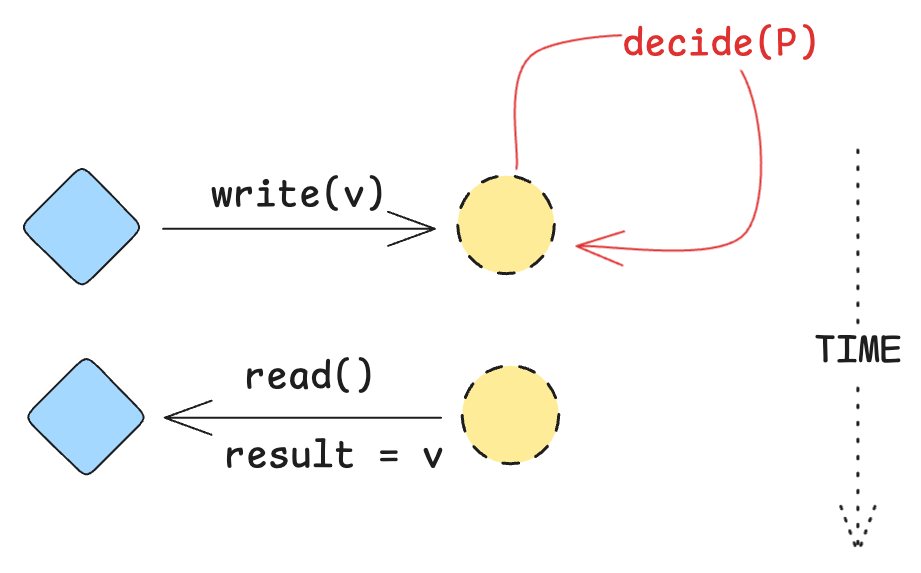
\includegraphics[width=0.30\textwidth]{general-problems/assets/flp-single-node-read-write.png}
    \caption{The single node case of read and write}
    \label{fig:flp-single-node-read-write}
\end{wrapfigure}

Let's begin with a setting which is not distributed in nature. Consider a client process $\verb|CL|$ and a server node $S$. The server $S$ saves a single bit value with itself and presents two distinct operations to the client $\verb|CL|$: 
\begin{itemize}
    \item \code{write(v: 0/1)}: This operation writes the value of a variable given by client at the server $S$.
    \item \code{read() $\to$ 0/1}: This operation returns the value of a variable stored at the server $S$.
\end{itemize}

A crucial component in this system is existence of a function $\verb|decide()|$, which can be anything that operates on the internal state of the server. A simplest form of $\verb|decide()|$ could be a function that returns the latest value stored in the server. Another variant could be a function that returns the XOR value of the last $5$ writes.

In our case, we can extend the same construction but to a distributed system outwardly presenting itself as a unit but internally being composed of multiple servers called \textbf{node}s. In essence, we desire that the same $\verb|write()|$, $\verb|read()|$ and $\verb|decide()|$ functions that were present in the single node case, be present in the distributed system as well and \textbf{they should act exactly the same}.

The FLP paper imagines the distributed setting to be describable as follows:

There are $n$ nodes in the distributed system. The nodes are connected to each other in connected but not necessarily a complete way in a graph-theoretic sense (a.k.a between any two nodes a path exist but not necessarily of length 1). Each process $p_i$ is defined by $p_i = (I_i, O_i, f_i)$ where $I_i$ is input in the set $\{0, 1\}$, $O_i$ is a one-time write only output in the set $\{\phi, 0, 1\}$, $\phi$ being the value it exercise if it has not yet been written to, and $f_i$ is a deterministic function that defines the internal state transition algorithm of $p_i$.

Each process $p_i$ can send a message $m \in M$ ($M$ being the "message universe") to some other process $p_x$ at any time as a tuple $(p_x, m)$ submitted to a globally singleton multi-set \textbf{message buffer} (note, source $p_i$ is not described in the tuple).

\index{Message Buffer}
The \textbf{message buffer} is a special non-deterministic (the only component in the system that is not deterministic) entity that presents each process with a function \code{receive(i) $\to$ $\{\phi, m\}$}. This function when called with index $i$, either returns $\phi$, a null message or $m$, one of the messages the buffer has received for delivery to process $p_i$. In the latter case, upon delivering the message, a tuple $(p_i, m)$ is removed from the message buffer. Note how message buffer sufficiently describes an asynchronous message passing system. It can choose to returen the null message any number of times, in effect simulating unbounded delay.

In a \textbf{synchronous} setting however, we have some upper bound on the time it takes for a message to be delivered. In an \textbf{asynchronous} setting, we have no such bound. As such, it is impossible to detect if the counterparty process has failed or is just taking a long time to respond.

One should also discuss a bit about what it means to "fail" in a distributed system. Typically we categorize failures in 4 different categories:
\begin{itemize}
    \item \textbf{Fail-stop}: The process halts, notifies everyone of its death and does not respond to any further messages.
    \item \textbf{Crash}: The process halts, does not notify anyone of its death and does not respond to any further messages.
    \item \textbf{Byzantine}: The process can send arbitrary messages to other processes, including lying about its own state.
    \item \textbf{Permissionless Byzantine}: The process can send arbitrary messages to other processes, including but not limited to impersonating a third-party.
\end{itemize}

In context of the FLP paper, we are concerned with the second type of failure, the "crash" without notification.

We define a \textbf{System Configuration $C$} as a unique combination of the internal states of all processes and the messages in the message buffer.

\subsection{Consensus, System Configurations, Events and Schedules}
Consensus in distributed systems is defined as any algorithm that satisfies the following properties:
\begin{itemize}
    \item \textbf{Agreement}: All non-faulty processes decide on the same value.
    \item \textbf{Termination}: All non-faulty processes eventually decide on a value.
    \item \textbf{Validity}: All non-faulty processes decide on a value that was some process's internal state at the start. \emph{Corollary}: If all non-faulty processes start with the same input value, then the decision value must be the same as the input value.
\end{itemize}

The system configuration $C$ advances to a new configuration $C'$ when it encounters \textbf{events}. 

\textbf{Events} are messages $(p, m)$ from the message buffer. Since there are many different messages that can be extracted from $C$ due to message buffer being non-deterministic, many different configurations can stem out from single configuration $C$. A list of events extracted from $C$ is called a \textbf{schedule}.

If at any system configuration $C$, all schedules lead to a final terminating consensus decision of value $v$, then we say that the system configuration $C$ is \textbf{decisive} / \textbf{univalent} for value $v$. This can also be written as \emph{v-valent}. Since we are in binary domain, decisive configurations are either $0$-valent or $1$-valent.

If at any system configuration $C$, different schedules lead to different consensus decisions, then we say that system configuration $C$ is \textbf{indecisive} / \textbf{multivalent}. Since we in binary domain, it also is called \emph{bi}-valent.

\subsection{Lemma 1: Disjoint Schedules Commute}
\begin{wrapfigure}{r}{0.20\textwidth}
    \centering
    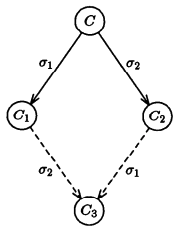
\includegraphics[width=0.20\textwidth]{general-problems/assets/flp-impossibility-lemma1.png}
    \caption{Schedules applying to disjoint processes can be out of order}
    \label{fig:flp-impossibility-lemma1}
\end{wrapfigure}
Suppose that from some configuration $C$, the schedules $\sigma_1$, $\sigma_2$ lead to configurations $C_1$, $C_2$ respectively. If the sets of processes taking steps in $\sigma_1$ and $\sigma_2$, respectively, are disjoint, then $\sigma_2$ can be applied to $C_1$ and $\sigma_1$ can be applied to $C_2$, and both lead to the same configuration $C_3$. See \ref{fig:flp-impossibility-lemma1} for a visual representation.

\subsection{Lemma 2: There exists a bi-valent initial configuration}

Let us assume the contrary to be the case, i.e. all initial system configurations C are decisive, uni-valent. Then, either all are 0-valent, 1-valent or a mix of both with some states being 0-valent and others 1-valent.

A strictly 0-valent or 1-valent configuration is trivial in nature and does not require any consensus protocol to reach a decision. However, a mix of both 0-valent and 1-valent configurations would require a consensus protocol to reach a decision.

Assume $n$ processes participating in the system. Then, all decisive initial configurations are $2^n$ in number. Since all of them are uni-valent. There would exist some adjecency boundary between 0-valent and 1-valent configurations in the $n$ dimensional lattice, the only process differentiating this being one of the $n$ processes in the system. If such process goes down without notice, the system would be left in a bi-valent state if it intends to resolve the consensus deterministically as it cannot choose 0-valency or 1-valency.

\subsection{Lemma 3: All roads lead to indecision}
\textbf{Claim}: If we start from some bi-valent system configuration $C_i$, with some specific event $e = (p, m)$ extractable from the message buffer from $C_i$, there exists a schedule $S_{C_i}$ that leads to a bi-valent configuration $C_{i+1}$ with event $e$ consumed in the process.

\begin{figure}[H]
    \centering
    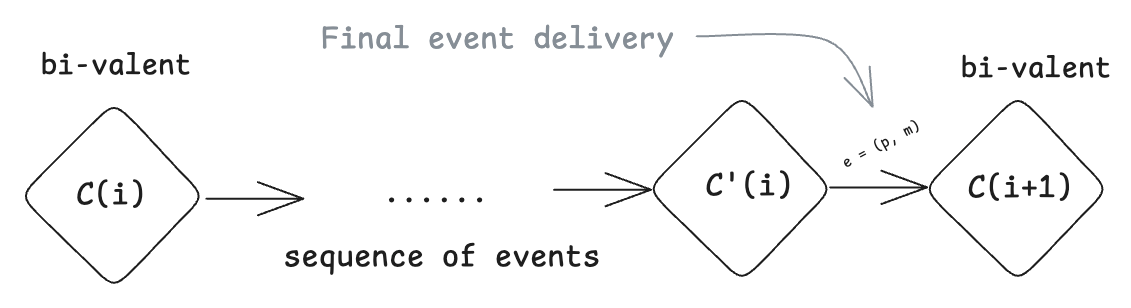
\includegraphics[width=0.7\textwidth]{general-problems/assets/flp-sequence-bivalent-to-bivalent.png}
    \caption{A bi-valent configuration can lead to another bi-valent configuration}
    \label{fig:bivalent-to-bivalent}
\end{figure}

It is noteworthy that we operate in a asynchronous network model, where-in while it can take a really long time for a message to be delivered, the guarantee exists that it is eventually delivered.

This lemma intends to present that there is a sequence of message deliveries that we can do at each bi-valent configuration that leads to another bi-valent configuration, and also that $e$ getting delivered. Multiple applications of this approach will essentially prove the FLP impossibility theorem.

Let us set-up the proof in the following way:
\begin{itemize}
    \item Start with a bi-valent configuration $C_i$.
    \item Let there be a sequence of events $S_{C_i} = \{e_1, e_2, \ldots, e_n\}, e_i \ne e \forall i \in [0, n]$ that lead to a bi-valent configuration $C_{i+1}$. It should be noted that $|S_{C_i}| = 0$ is possible.
    \item Let $C'_{i}$ be the "penultimate configuration" that is reached by applying the schedule $S_{C_i}$ to $C_i$. Since $|S_{C_i}| = 0$ is possible, $C'_{i}$ can be the same as $C_i$.
\end{itemize}

\textbf{All configurations in \ref{fig:bivalent-to-bivalent} are bi-valent}: It is easy to see that in our definition of system configurations, we can never go from a uni-valent configuration to a bi-valent configuration. In this setup of $C_i$ and $C_{i+1}$ both being bi-valent, all the intermediate configurations including the penultimate configuration $C'_{i}$ must also be bi-valent.

We now define a few possible configuration categories for intermediate and penultimate configurations shown in \ref{fig:bivalent-to-bivalent}.

\begin{itemize}
    \item \textbf{Pre-uni-valent}: Some configuration $C^*$ is pre-uni-valent, if it is reachable from $C_i$ via some sequence of events without delivering $e = (p, m)$ and application of $e$ to it would transition into a new configuration $C^{**}$ which will be uni-valent. For example, if $C'$ is pre-uni-valent, then $C_{i+1}$ is uni-valent which we do not want.
    \item \textbf{Pre-bi-valent}: Some configuration $C^*$ is pre-bi-valent, if it is reachable from $C_i$ via some sequence of events without delivering $e = (p, m)$ and application of $e$ to it would transition into a new configuration $C^{**}$ which will be bi-valent. For example, if $C'$ is pre-bi-valent, then $C_{i+1}$ is uni-valent which we want.
\end{itemize}

Note that Pre-X-valency resolving into X-valency for X being uni or bi, is a property of the event $e = (p, m)$.

Note that all Pre-uni-valent configurations necessarily need to be bi-valent. As by definition, at that configuration if a decision is already made, the configuration would reduce to uni-valency. Hence, a Pre-0-valent configuration will have both 0-valent and atleast one of 1-valent and bi-valent configurations as its reachable children configurations. Similar argument goes for Pre-1-valent (atleast one of 0-valent or bi-valent) and Pre-bi-valent (atleast one of 0-valent or 1-valent).

So, what can we say about $C_i$? Well, if $C_i$ is Pre-bi-valent, then by definition application of $e$ to it will lead to a bi-valent configuration $C_{i+1}$. In this case, we have proven bi-valency leading to bi-valency.

The other case however is more interesting. What if $C_i$ is Pre-uni-valent? Well, direct application of $e$ to it will lead to a uni-valent configuration which we want to avoid. We need to path our way from a Pre-uni-valent configuration $C_i$ to some Pre-bi-valent $C'_{i}$ so that we can transition into a bi-valent $C_{i+1}$ by application of $e$. \textbf{Can we always path a way from a Pre-uni-valent configuration to a Pre-bi-valent configuration?}

We begin with an assumption that $C_i$ is Pre-0-valent. Assume another event $e' = (p', m')$ distinct from $e = (p, m)$ such that application of $e'$ to some reachable configuration $X$ from $C_i$ leads to a non Pre-0-valent configuration $Y$. See figure \ref{fig:finding-non-pre-0-valent} for a visual representation.

\begin{figure}[H]
    \centering
    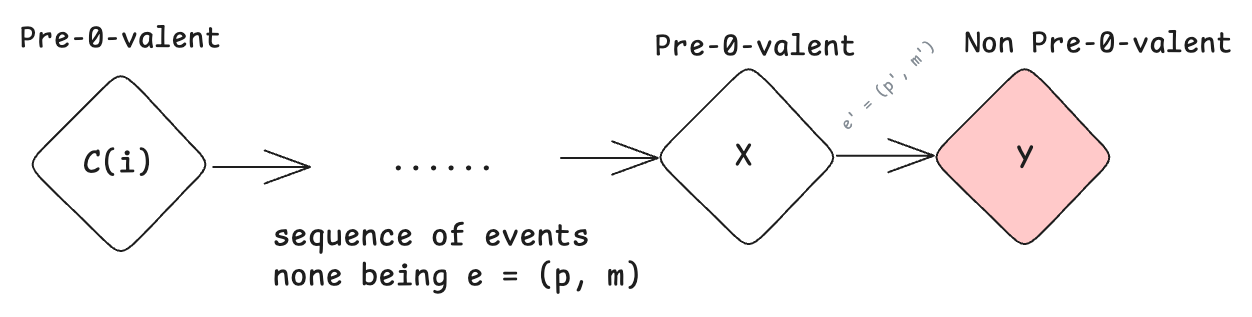
\includegraphics[width=0.7\textwidth]{general-problems/assets/flp-pre-0-valent-to-non-pre-0-valent.png}
    \caption{Finding a non Pre-0-valent configuration from a Pre-0-valent configuration}
    \label{fig:finding-non-pre-0-valent}
\end{figure}

We claim to \textbf{show that $Y$ is Pre-bi-valent}.

This is because, if $Y$ is Pre-1-valent and $e$ is applied to it, the resulting configuration $Y'$ will be 1-valent. However, since $e$ can be applied to $X$ as well, the resulting $X'$ from $X$ will be 0-valent. If later on, $e'$ is applied to $X'$, the resulting configuration $X''$ will also be 0-valent.

However, we note that $X''$ is identical to $Y'$ by lemma 1 if $e$ and $e'$ are disjoint, i.e. $p' \ne p$. This is a contradiction as $Y'$ is 1-valent and $X''$ is 0-valent.

On the other hand if $p' = p$, then resolution of deterministic value of choice rests on a single process $p$. If this process crashes, the system will be left in a bi-valent state.

Hence, under the assumption of possibility of single node failure, transition from Pre-0-valency to Pre-1-valency is impossible. This implies that $Y$ indeed is a Pre-bi-valent configuration.

\subsection{Proving the theorem}
Let us start our protocol from some initial bi-valent configuration $C_0$. Existence of such initial configuration is given by lemma 2.

For any transition to $C_{i+1}$ from $C_{i}$, we choose the oldest message $e_{old}$ known to be in the message buffer at $C_i$. Given $C_i$ and $e_{old}$, we can construct a schedule $S_{C_i}$ that leads to $C_{i+1}$ as per lemma 3 leading to a bi-valent configuration. This also, leads to the consumption of the oldest message $e_{old}$ known at $C_i$.

We continously apply the above scheme till the point we are left with no messages in the message buffer. We eventually still reach a bivalent state $C_{\infty}$.

\subsection{Conclusion}
\begin{itemize}
    \item The FLP impossibility theorem makes clear that \textbf{trade-offs are required} in the design of distributed systems. Whether it is loosening up on deterministic guarantees or on tightening up on timing guarantees, you cannot have both.
    \item The above can also be described as, in event of asynchrony, do you compromise on consistency (determinism) or on liveness? \textbf{Longest chain (Nakamoto) based consensus protocols like Bitcoin and Ethereum compromise on consistency, while protocols like PBFT compromise on liveness}.
\end{itemize}

\begin{refbox}{Further Resources}
    \small
    \begin{description}
        \item [Original Paper]: \href{https://groups.csail.mit.edu/tds/papers/Lynch/jacm85.pdf}{https://groups.csail.mit.edu/tds/papers/Lynch/jacm85.pdf}
        \item [Overview - FLP Impossibility Theorem]: \href{https://www.youtube.com/watch?v=Vmlj-67aymw}{https://www.youtube.com/watch?v=Vmlj-67aymw}
        \item [Extending the bi-valent configuration (Lemma 3)]: \href{https://www.youtube.com/watch?v=cwEXmcszbos}{https://www.youtube.com/watch?v=cwEXmcszbos}
        \item [Consize summary]: \href{https://www.youtube.com/watch?v=2fnS-f-mwIo}{https://www.youtube.com/watch?v=2fnS-f-mwIo}
    \end{description}
\end{refbox}